\documentclass[a4paper,12pt]{article} % тип документа

% Поля страниц
\usepackage[left=2.5cm,right=2.5cm, top=2cm,bottom=2cm,bindingoffset=0cm]{geometry}
    
%Пакет дял таблиц   
\usepackage{multirow} 
    
%Отступ после заголовка    
\usepackage{indentfirst}


% Рисунки
\usepackage{subcaption,floatrow,graphicx,calc}
\usepackage{wrapfig}

% Создаёем новый разделитель
\DeclareFloatSeparators{mysep}{\hspace{1cm}}

% Ссылки?
\usepackage{hyperref}
\usepackage[rgb]{xcolor}
\hypersetup{				% Гиперссылки
    colorlinks=true,       	% false: ссылки в рамках
	urlcolor=blue          % на URL
}


%  Русский язык
\usepackage[T2A]{fontenc}			% кодировка
\usepackage[utf8]{inputenc}			% кодировка исходного текста
\usepackage[english,russian]{babel}	% локализация и переносы

\usepackage{siunitx}


% Математика
\usepackage{amsmath,amsfonts,amssymb,amsthm,mathtools, mathrsfs, wasysym}

\title{\textbf{эффект Рамзауэра} (5.1.3)}
\author{Манро Эйден Б01-303б}
\date{}

\begin{document}

\maketitle

\noindent \textbf{Цель работы}: получить ВАХ эффекта на экране осциллографа; измерить расстояние между характерными точками в вольтах; снять ВАХ в статическом режиме; по результатам измерений рассчитать размер электронной оболочки атома, оценить глубину потенциальной ямы и потенциал ионизации атома, заполняющего лампу.

\begin{center}
\section*{Теоретическая часть}
\end{center}
    
\subsection*{Основная идея}

Эффект Рамзауэра наблюдается при упругом рассеянии электронов с энергией порядка $\sim 10$ эВ на атомах инертных газов, например аргона.
Классическая теория предсказывает, что вероятность рассеяния должна монотонно убывать с ростом энергии электрона, однако эксперимент показывает наличие энергий, при которых рассеяние почти отсутствует.

С точки зрения квантовой механики электрон ведёт себя как волна де Бройля. При попадании внутрь атома часть его энергии превращается в потенциальную, и скорость электрона изменяется. Это приводит к изменению длины волны, и по отношению к электронной волне атом начинает играть роль преломляющей среды с показателем

\begin{equation}
    n = \sqrt{1 - \frac{U}{E}},
\end{equation}

где $U$ — потенциальная энергия внутри атома, $E$ — полная энергия электрона.

\subsection*{Модель прямоугольной ямы}

Для количественного описания эффекта атом можно заменить на одномерную потенциальную яму прямоугольной формы шириной $l$ и глубиной $U_0$.
Решение уравнения Шрёдингера для такой системы приводит к выражению для коэффициента прохождения электрона:

\begin{equation}
    \frac{1}{D} = 1 + \frac{U\_0^2}{4 E (E+U_0)} \sin^2(k_2 l),
\end{equation}

где волновое число внутри ямы равно

\begin{equation}
    k_2 = \sqrt{\frac{2 m (E+U_0)}{\hbar^2}}.
\end{equation}

Из формулы видно, что коэффициент прохождения зависит от энергии электрона периодически. Минимум рассеяния (так называемое «просветление атома») достигается при выполнении условия

\begin{equation}
k_2 l = \pi n, \quad n \in \mathbb{N}.
\end{equation}

\subsection*{Интерференция волн де Бройля}

То же самое условие можно получить и из волновой интерпретации: в атоме происходит интерференция волны, прошедшей через потенциальную яму, и волны, отражённой от её границ.
При определённых энергиях возникает полное гашение отражённой волны, что соответствует минимуму рассеяния.

Энергии электронов при первом максимуме и минимуме коэффициента прохождения связаны с размерами атома следующими соотношениями:

\begin{equation}
2 l = \frac{h}{\sqrt{2 m (E_1 + U_0)}}, \qquad
2 l = \frac{3h}{2\sqrt{2 m (E_2 + U_0)}}.
\end{equation}

Из этих выражений можно исключить одну из величин и получить формулы для эффективной ширины атома и глубины потенциальной ямы:

\begin{equation}
l = \frac{h \sqrt{5}}{\sqrt{32 m (E_2 - E_1)}}, \qquad
U_0 = \frac{4}{5} E_2 - \frac{9}{5} E_1.
\end{equation}

\subsection*{Вероятность рассеяния}

Для перехода от теоретической модели к эксперименту необходимо связать вероятность рассеяния с наблюдаемыми величинами.
Измеряя анодный ток \$I(U)\$ при различных ускоряющих напряжениях \$U\$, можно вычислить вероятность рассеяния электронов по формуле

\begin{equation}
w(U) = -\frac{1}{C} \ln \frac{I(U)}{I_0},
\end{equation}

где $I_0$ — катодный ток (ток без рассеяния), а $C$ — постоянная, зависящая от геометрии прибора.

Таким образом, построив график $w(U)$ по экспериментальной ВАХ, можно непосредственно наблюдать энергетическую зависимость вероятности рассеяния и убедиться в существовании эффекта Рамзауэра.


\begin{center}
\section*{Экспериментальная установка}
\end{center}
    
В нашей для изучения эффекта Рамзауэра используется тиратрон ТГ3-01/1.3Б, заполненный инертным газом. Схематическое изображение тиратрона и его конструкция приведены на рис.~\ref{setup}.

Схема установки для изучения эффекта Рамзауэра приведена на рис.~\ref{scheme}. На лампу Л подаётся синусоидальное напряжение частоты 50 Гц от источника питания ИП, С -- стабилизированный блок накала катода; исследуемый сигнал подаётся на электронный осциллограф (ЭО); цифрами обозначены номера ножек лампы.

\thisfloatsetup{floatrowsep=mysep}	
\begin{figure}[h!]
    \ffigbox{
        \begin{subfloatrow}[2]
            \ffigbox[\FBwidth]{\caption{}}%
            {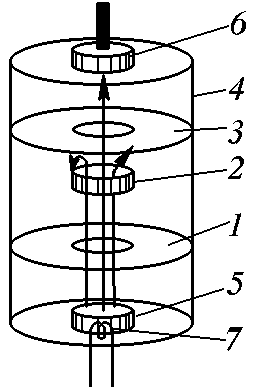
\includegraphics[width=3cm,height=4.5cm]{setup.png}{\label{setup}}}
            \ffigbox[\FBwidth]{\caption{}}%
            {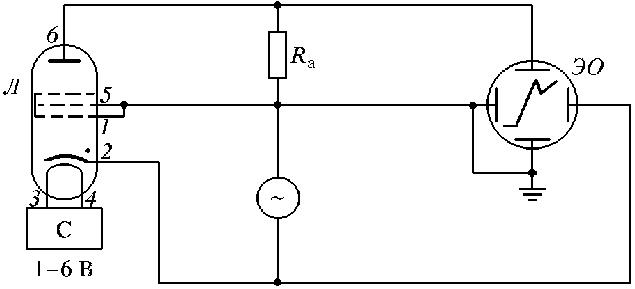
\includegraphics[width=7cm,height=4cm]{scheme.png}{\label{scheme}}}         
        \end{subfloatrow}
    }
    {\caption{Экспериментальная установка.}}
\end{figure}

Схема экспериментальной установки, изображённая на рис.~\ref{scheme} в нашей работе конструктивно осуществлена следующим образом. Лампа-тиратрон ТГ3-01/1.3Б, заполненная инертным газом, расположена непосредственно на корпусе блока источника питания (БИП). Напряжение к электродам лампы подаётся от источников питания, находящихся в корпусе прибора. Регулировка напряжения и выбор режима работы установки производится при помощи ручек управления, выведенных на лицевую панель БИП.

\newpage

\begin{center}
    \section*{Обработка данных}
\end{center}

\subsection*{Динамический режим}

\floatsetup[table]{capposition=top}	
		\begin{table}[H]
			\caption{Измеренные величины в динамическом режими}
			\label{table:parametr}
			\begin{tabular}{|c|c|c|c|c|}
				\hline
				$U_{накакала}$, В & $V_{max}$, эВ & $V_{min}$, эВ & $V_{\text{пробоя}}, эВ $ \\ \hline
                2.98 $\pm$ 0.01 & 1.6 $\pm$ 0.4  & 5.8 $\pm$ 0.4 & 11.6 $\pm$ 0.4   \\ \hline
                
			\end{tabular}
		\end{table}

Радиус атома ядра:
$$
    l = (3.34 \pm 0.8) \; \si{\angstrom}
$$

Глубина потенциальной ямы:
$$
    U_0 = (3.92 \pm 1.23) \; \text{В}
$$
        
\subsection*{Статический режим}

\floatsetup[table]{capposition=top}	
		\begin{table}[H]
			\caption{Измеренные величины в статическом режими}
			\label{table:parametr}
			\begin{tabular}{|c|c|c|c|}
				\hline
				$U_{накакала}$, эВ & $V_{max}$, эВ & $V_{min}$, эВ  \\ \hline
                2.99 $\pm$ 0.01 & 1.76 $\pm$ 0.04 & 5.62 $\pm$ 0.04   \\ \hline
                
			\end{tabular}
		\end{table}

Нахождение экстремумов анодного напряжение осуществлялся методом аппроксимации параболой по нечетным и четным точкам.


Радиус атома ядра:
$$
    l = (3.48 \pm 0.09) \; \si{\angstrom}
$$

Глубина потенциальной ямы:
$$
    U_0 = (4.44 \pm 0.14) \; \text{В}
$$

\begin{figure}[h!]
    \begin{center}
    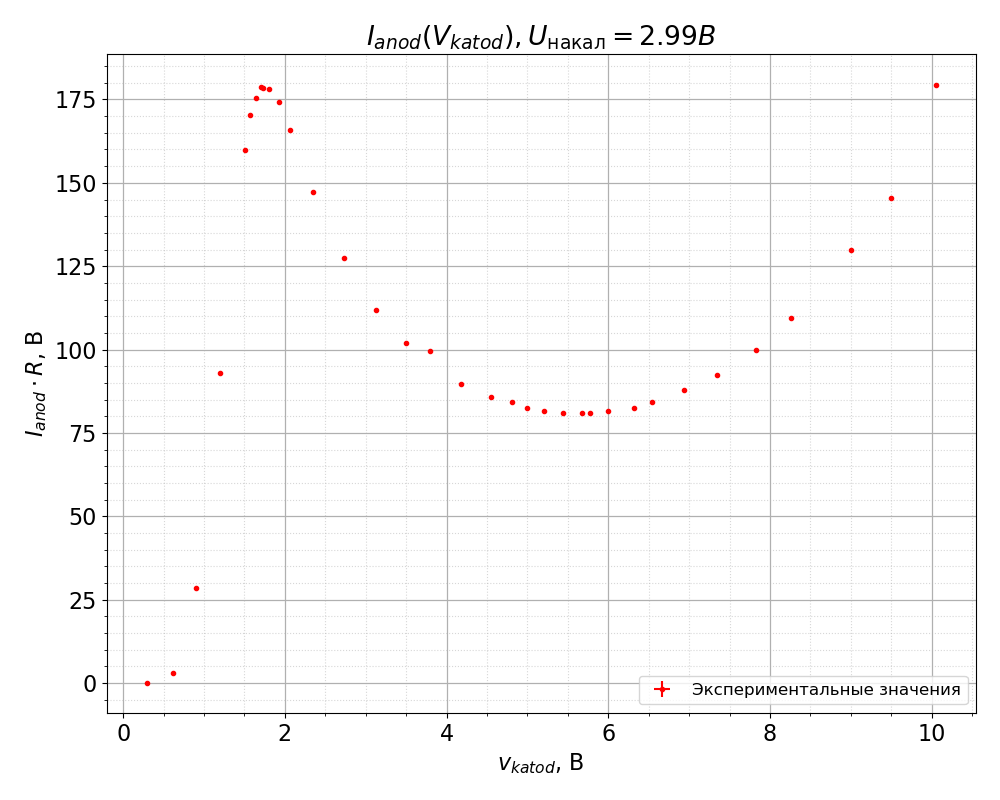
\includegraphics[width = 0.8\textwidth]{I(V).png}
    \caption{Зависимость $I(V)$}
    \end{center}
\end{figure}

\begin{figure}[h!]
    \begin{center}
    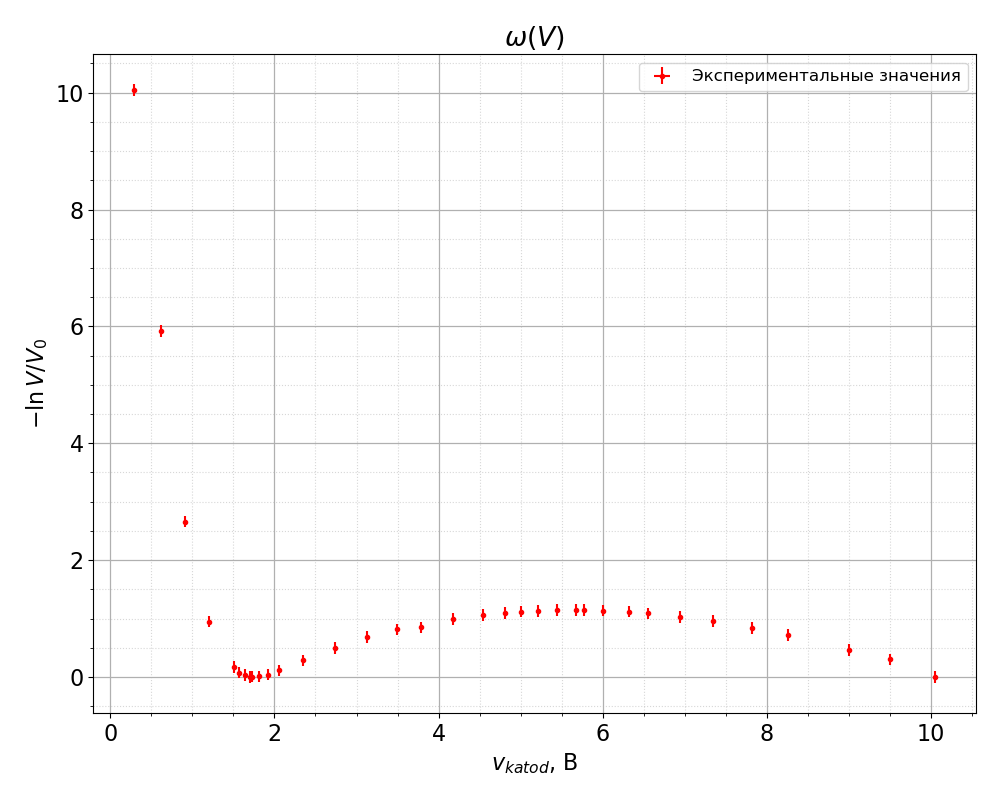
\includegraphics[width = 0.8\textwidth]{w(V).png}
    \caption{Зависимость $w(V)$}
    \end{center}
\end{figure}

\newpage

\begin{center}
\section*{Вывод}
\end{center}

В ходе эксперимента был подтверждён эффект Рамзауэра, проявляющийся в наблюдении минимума сечения рассеяния электронов на атомах ксенона. По статическим вольт-амперным характеристикам были определены основные параметры модели: средняя длина свободного пробега и эффективная глубина потенциальной ямы.

Расчёт по интерференционной модели показал, что максимумы коэффициента прохождения должны наблюдаться при энергиях $E_1 \approx 2.5$ эВ, $E_2 \approx 12.1$ эВ, $E_3 \approx 28.1$ эВ. Отсутствие второго максимума в экспериментальных данных объясняется его близостью к энергии ионизации атома аргона.

Качественное согласие с теорией подтверждается эквивалентностью зависимостей $\omega(V) = -\ln(V/V_0)$ и $-\ln(I/I_0)$, а также наблюдением экстремумов на близких напряжениях в статическом и динамическом режимах. Данный факт, наряду с наличием минимума рассеяния, является прямым доказательством волновой природы электрона и его способности интерферировать при рассеянии на потенциале, что полностью соответствует предсказаниям квантовой механики.

Надёжность статического метода измерения оказалась выше динамического, так как он позволяет получить меньшую относительную погрешность за счёт отсутствия инерционности измерительной цепи и обеспечивает более точное определение положений экстремумов ВАХ.

Следует отметить, что использованные модели справедливы для описания рассеяния электронов с энергией $E \gtrsim 1$ эВ. При меньших энергиях начинают проявляться другие квантовые эффекты, такие как резонансное рассеяние медленных электронов.
        
				
\end{document}